\section{Other}
\subsection*{Causal Models}
\emph{Basics} ---
\begin{itemize}
    \item Correlation / prediction does not necessarily imply causality, but causality necessarily implies correlation / predictability
    \item If $A$ and $O$ are correlated, there are $4$ possibilities:
    \begin{itemize}
        \item \emph{Chain}:
        \begin{itemize}
            \item $A$ causes $O$
            \item $O$ causes $A$
        \end{itemize}
        \item \emph{Fork}:
        \begin{itemize}
            \item $A$ and $O$ have a common cause $C$
        \end{itemize}
        \item $A$ and $O$ do not have a causal relationship and are correlated by chance
    \end{itemize}
    \item If upon intervention $A$, $O$ happens, there are $3$ possibilities:
    \begin{itemize}
        \item $A$ directly causes $O$, i.e., $O$ happens upon intervention $A$ if all other variables are kept constant
        \item $A$ indirectly causes $O$, i.e., $O$ happens upon intervention $A$ if all prior and simultaneous variables are kept constant
        \item $A$ does not cause $O$, i.e., $O$ does not happen upon intervention $A$ if all prior and simultaneous variables are kept constant
    \end{itemize}
    \item Causality can be inferred only when controlling for all prior and simultaneous variables
    \item If we want to model the causal relationship between $A$ and $O$, we need to consider the following:
    \begin{itemize}
        \item $A$ might be imperfectly correlated with $B$, which also (in)directly affects $O$:
        \begin{itemize}
            \item Regression coefficient for $A$ can carry unwanted proxy effects of $B$ if used alone in a model. Instead, it is desirable to single out direct effects of each factor if all other prior and simultaneous variables are kept constant
            \item Options:
            \begin{itemize}
                \item Chain:
                \begin{itemize}
                    \item $A$ causes $B$
                    \item $B$ causes $A$
                \end{itemize}
                \item Fork:
                \begin{itemize}
                    \item $A$ and $B$ have a common cause $C$
                \end{itemize}
                \item $A$ and $B$ do not have a causal relationship and are correlated by chance
            \end{itemize}
            \item \emph{Confounding variables} (i.e., prior variables that $A$ is caused by and simultaneous variables that $A$ is correlated with by chance, which also affect $O$) should be included in the model to avoid \emph{omitted variable bias}:
            \begin{itemize}
                \item Variable $B$, if it causes $A$
                \item Common cause $C$ of $B$ and $A$
                \item Variable $B$, if it has no causal relationship to $A$
                \item If variable $B$ only indirectly affects $O$, either variable $B$ or an intermediate between $B$ and $O$ can be included in the model
            \end{itemize}
            \item \emph{Intermediate} and \emph{collider variables} (i.e., variables caused by $A$ and $O$, creating a \emph{selection bias}) should be excluded from the model to avoid \emph{overcontrol} and \emph{endogenous selection bias}:
            \begin{itemize}
                \item Variable $B$, if it is caused by $A$
                \item Variable $D$, if it is caused by $A$ and $O$
            \end{itemize}
        \end{itemize}
        \item $A$ might be perfectly correlated with $B$, which also (in)directly affects $O$: Causal effects of each variable cannot be separated
        \item $A$ might be perfectly uncorrelated with $B$, which also (in)directly affects $O$:
        \begin{itemize}
            \item $A$ and $B$ do not have a causal relationship
            \item $B$ does not impact the regression coefficient for $A$ and can be excluded from the model
        \end{itemize}
        \item \emph{Shortcut learning}: $A$ might be spuriously correlated with $B$, which does not affect $O$
        \begin{itemize}
            \item Important to only encode $A$ in the features (i.e., generate an invariant representation), not $B$
            \item Aim is to represent counterfactually invariant relationships between $A$ and $O$, i.e., invariant to different counterfactuals represented by different states of $B$
        \end{itemize}
    \end{itemize}
\end{itemize}

\emph{Causal scenarios} --- 
\begin{itemize}
    \item \emph{Causal scenario without selection bias}: $\mathcal{X}$ affects $\mathcal{Y}$ and there is no selection bias. Features $\mathcal{X}$ can be grouped into:
    \begin{itemize}
        \item Features $\mathcal{X}_{\bot Y}$ do not causally affect $\mathcal{Y}$, but are affected by $\mathcal{W}$. These features have no causal relationship
        \item Features $\mathcal{X}_{\bot W}$ causally affect $\mathcal{Y}$, but are not affected by $\mathcal{W}$. These features have a direct causal relationship
        \item Features $\mathcal{X}_{W \& Y}$ causally affect $\mathcal{Y}$ and are affected by $\mathcal{W}$ (as well as $\mathcal{X}_{\bot Y}$ and $\mathcal{X}_{\bot W}$). These features link $\mathcal{W}$ and $\mathcal{Y}$ in a causal network
    \end{itemize}
    \item \emph{Anti causal scenario}: We assume $\mathcal{Y}$ affects $\mathcal{X}$, rather than the other way around
    \item \emph{Causal scenario with selection bias}: $\mathcal{X}$ affects $\mathcal{Y}$ and there is a selection bias 
\end{itemize}

{\color{lightgray}\hrule height 0.001mm}

\emph{Counterfactual invariance} --- 
\begin{itemize}
    \item Results of estimator remain consistent across different counterfactual scenarios, i.e. if $\mathcal{X} \to \mathcal{Y}$ and $\mathcal{W} \to \mathcal{X}$ but $\mathcal{W} \not\to \mathcal{Y}$ where $\to$ is a causal relationship, our estimator should be invariant to states of $\mathcal{W}$, i.e. $f(\mathcal{X}(\mathcal{W}_1)) = f(\mathcal{X}(\mathcal{W}_2))$
    \item For counterfactual invariance, the following must hold:
    \begin{itemize}
        \item Anti causal scenario: $(f(\mathcal{X}) \bot \mathcal{W}) | \mathcal{Y}$, i.e. estimate $f$ only depends on $\mathcal{X}_{\bot W}$, provided $\mathcal{Y}$ is known
        \item Causal scenario without selection bias, potentially with confoundedness: $f(\mathcal{X}) \bot \mathcal{W}$, i.e. estimate $f$ only depends on $\mathcal{X}_{\bot W}$
        \item Causal scenario without confoundedness, potentially with selection bias: $(f(\mathcal{X}) \bot \mathcal{W}) | \mathcal{Y}$ as long as $\mathcal{X}_{\bot Y}$ and $(\mathcal{Y} \bot \mathcal{X}) | \mathcal{X}_{\bot W}, \mathcal{W}$ 
    \end{itemize}
    \item We need to show:
    \begin{itemize}
        \item For causal scenario without selection bias we need to show: $\mathcal{X}_{\bot W} \bot \mathcal{W}$
        \item For anti causal scenario we need to show: $(\mathcal{X}_{\bot W} \bot \mathcal{W}) | \mathcal{Y}$
        \item This can be shown via \emph{d-separation}
    \end{itemize}
\end{itemize}

{\color{lightgray}\hrule height 0.001mm}

\emph{$D$ separation} --- 
\begin{itemize}
    \item Undirected path of $n$ nodes is \emph{d-separated}, if it contains 3 nodes following any of the following forms and if this form is \emph{blocked}: 
    \begin{itemize}
        \item \emph{Chain structure}: $X \rightarrow Z \rightarrow Y$ or $Y \rightarrow Z \rightarrow X$ – is blocked, if we condition on $Z$, i.e. $Z$ is known
        \item \emph{Fork structure}: $X \leftarrow Z \rightarrow Y$ – is blocked, if we condition on $Z$, i.e. $Z$ is known
        \item \emph{Collider structure}: $X \rightarrow Z \leftarrow Y$ – is blocked, if we don't condition on $Z$ or any of its descendants
    \end{itemize}
    \item Random variables $X$ and $Y$ are conditionally independent if each path between them is d-separated\\
    $\rightarrow$ as soon as we have one blocked triple on path, entire path is blocked\\
    $\rightarrow$ as soon as one path is active, we cannot guarantee conditional independence
    \item For causal scenario without selection bias we can show $\mathcal{X}_{\bot W} \bot \mathcal{W}$ since all paths are blocked 
    \item For anti causal scenario we can show $(\mathcal{X}_{\bot W} \bot \mathcal{W}) | \mathcal{Y}$ since all paths are blocked, conditioned on $\mathcal{Y}$, i.e. if $\mathcal{Y}$ is known
\end{itemize}

{\color{black}\hrule height 0.001mm}

\subsection*{Proofs}

\emph{Proofs} --- 
\begin{itemize}
    \item To prove $p \rightarrow q$:
    \begin{itemize}
        \item Prove $p \rightarrow \neg q$ is impossible
        \item Prove $\neg q \rightarrow \neg p$
    \end{itemize}
    \item To prove $p \leftrightarrow q$: Prove $p \rightarrow q$ and $q \rightarrow p$
    \item To prove statement by induction: 
    \begin{itemize}
        \item Prove base case for $n=0$ or $n=1$
        \item Assume inductive hypothesis: Assume statement holds for $n=k$
        \item Prove inductive step: Prove statement holds for $n=k+1$
    \end{itemize}
\end{itemize}

\textit{1) $D$ separation}\\
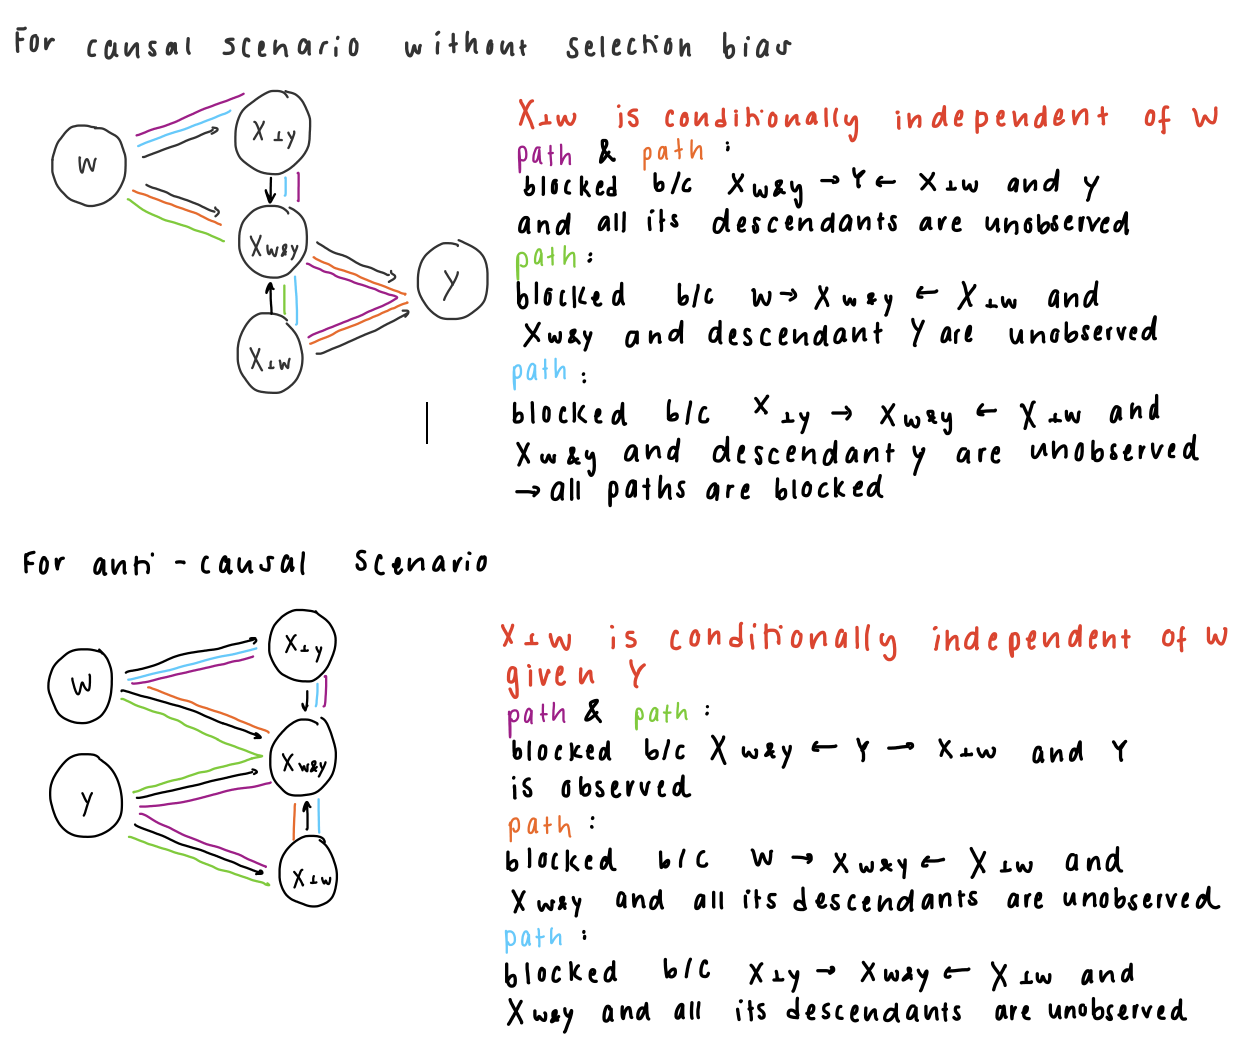
\includegraphics[height=25mm]{inhalt/images/99_other_1.png}